\documentclass{beamer}
\mode<presentation>
{
%  \usetheme[hideothersubsections]{PaloAlto}
  \usetheme{default}
  \setbeamercovered{transparent}
}

\usepackage[english]{babel}
\usepackage[latin1]{inputenc}

\usepackage{amsfonts}
\usepackage{amsmath}
\usepackage{fancyhdr}
\usepackage{hyperref}
\usepackage{tikz}
\usepackage{pgfplots}
\usepackage{listings}

\newcommand{\bbR}{\mathbb{R}}
\newcommand{\bbC}{\mathbb{C}}

\newcommand{\hdr}[2]{
  \pagestyle{fancy}
  \lhead{Bindel, Spring 2015}
  \rhead{Numerical Analysis (CS 4220)}
  \fancyfoot{}
  \begin{center}
    {\large{\bf #1}} \\
    Due: #2
  \end{center}
  \lstset{language=matlab,columns=flexible}
}

\newcommand{\phdr}[1]{
  \pagestyle{fancy}
  \lhead{Bindel, Spring 2015}
  \rhead{Numerical Analysis (CS 4220)}
  \fancyfoot{}
  \begin{center}
    {\large{\bf #1}}
  \end{center}
  \lstset{language=matlab,columns=flexible}
}


\newcommand{\shdr}[2]{
  \title[CS 4220, Fall 2014]{#1}
  \author[]{David Bindel} \date[]{#2}
}

\lstset{language=matlab,columns=flexible}  


\shdr{Whirlwind Tour of LA \\ Part 1: Some Nitty-Gritty Stuff}{2015-01-30}

\begin{document}

\begin{frame}
  \titlepage
\end{frame}

\begin{frame}
  \frametitle{Logistics}

  \begin{itemize}
  \item PS1/2 deferred to next Weds/Fri
    \begin{itemize}
    \item Brandon has OH tonight 5-7
    \item I will arrange extra OH early next week (TBA)
    \end{itemize}
  \item Please keep up with the reading!
  \item Ask me questions!
  \end{itemize}
\end{frame}

\begin{frame}
  \frametitle{Big picture: What's a matrix?}

  An array of numbers, or a representation of
  \begin{itemize}
  \item A tabular data set?
  \item A graph?
  \item A linear function between vector spaces?
  \item A bilinear function on two vectors?
  \item A pure quadratic function?
  \end{itemize}
  It's all the above, plus being an interesting object on its own!

  \vspace{5mm}
  Let's start concrete.
  
\end{frame}

\begin{frame}[fragile]
  \frametitle{Basics: Constructing matrices and vectors}

  \begin{lstlisting}
    x = [1; 2];       % Column vector
    y = [1, 2];       % Row vector
    M = [1, 2; 3, 4]; % 2-by-2 matrix
    M = [I, A];       % Horizontal matrix concatenation
  \end{lstlisting}
\end{frame}

\begin{frame}[fragile]
  \frametitle{Basics: Constructing matrices and vectors}

  \begin{lstlisting}
    I = eye(n);    % Build n-by-n identity
    Z = zeros(n);  % n-by-n matrix of zeros
    b = rand(n,1); % n-by-1 random matrix (uniform)
    e = ones(n,1); % n-by-1 matrix of ones
    D = diag(e);   % Construct a diagonal matrix
    e2 = diag(D);  % Extract matrix diagonal
  \end{lstlisting}
\end{frame}


\begin{frame}[fragile]
  \frametitle{Basics: Transpose, rearrangements}

  \begin{lstlisting}
    % Reshape A to a vector, then back to a matrix
    % Note: MATLAB is column-major
    avec = reshape(A, prod(size(A)));
    A = reshape(avec, n, n);
    
    A = A';  % Conjugate transpose
    A = A.'; % Simple transpose

    idx = randperm(n);  % Random permutation of indices
    Ac = A(:,idx);      % Permute columns of A
    Ar = A(idx,:);      % Permute rows of A
    Ap = A(idx,idx);    % Permute rows and columns
  \end{lstlisting}
\end{frame}

\begin{frame}[fragile]
  \frametitle{Basics: Submatrices, diagonals, triangles}
  
  \begin{lstlisting}
    A = randn(6,6);   % 6-by-6 random matrix
    A(1:3,1:3)        % Leading 3-by-3 submatrix
    A(1:2:end,:)      % Rows 1, 3, 5
    A(:,3:end)        % Columns 3-6
    
    Ad = diag(A);       % Diagonal of A (as vector)
    A1 = diag(A,1);     % First superdiagonal
    Au = triu(A);       % Upper triangle
    Al = tril(A);       % Lower triangle
  \end{lstlisting}
\end{frame}

\begin{frame}[fragile]
  \frametitle{Basics: Matrix and vector operations}
  
  \begin{lstlisting}
    y = d.*x;   % Elementwise multiplication of vectors/matrices
    y = x./d;   % Elementwise division
    z = x + y;  % Add vectors/matrices
    z = x + 1;  % Add scalar to every element of a vector/matrix
    
    y = A*x;    % Matrix times vector
    y = x'*A;   % Vector times matrix
    C = A*B;    % Matrix times matrix

    % Don't use inv!
    x = A\b;    % Solve Ax = b *or* least squares
    y = b/A;    % Solve yA = b or least squares
  \end{lstlisting}
\end{frame}

\begin{frame}
  \frametitle{Two basic operations}

  \begin{itemize}
  \item Matrix-vector product (matvec): $O(n^2)$
  \item Matrix-matrix product (matmul): $O(n^3)$
  \end{itemize}
\end{frame}

\begin{frame}
  \frametitle{Matvec}

  A matvec is a collection of dot products.
  \begin{center}
  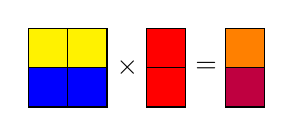
\begin{tikzpicture}[scale=0.5]
    \begin{scope}
      \draw[fill=blue]   (0,0) rectangle (2,1);
      \draw[fill=yellow] (0,1) rectangle (2,2);
      \draw[fill=red]    (3,0) rectangle (4,2);
      \draw[fill=purple] (5,0) rectangle (6,1);
      \draw[fill=orange] (5,1) rectangle (6,2);
      \draw(0,0) grid (2,2);
      \draw(3,0) grid (4,2);
      \draw(5,0) grid (6,2);
      \node[right] at (2,1) {$\times$};
      \node[right] at (4,1) {$=$};
    \end{scope}
  \end{tikzpicture}
  \end{center}

  A matvec is a sum of scaled columns.
  \begin{center}
  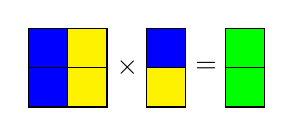
\begin{tikzpicture}[scale=0.5]
    \begin{scope}
      \draw[fill=blue]   (0,0) rectangle (1,2);
      \draw[fill=yellow] (1,0) rectangle (2,2);
      \draw[fill=yellow] (3,0) rectangle (4,1);
      \draw[fill=blue]   (3,1) rectangle (4,2);
      \draw[fill=green]  (5,0) rectangle (6,2);
      \draw(0,0) grid (2,2);
      \draw(3,0) grid (4,2);
      \draw(5,0) grid (6,2);
      \node[right] at (2,1) {$\times$};
      \node[right] at (4,1) {$=$};
    \end{scope}
  \end{tikzpicture}
  \end{center}

  Can also think of {\em block} rows/columns.
  \begin{center}
  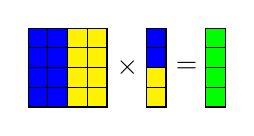
\begin{tikzpicture}[scale=0.25]
    \begin{scope}
      \draw[fill=blue]   (0,0) rectangle (2,4);
      \draw[fill=yellow] (2,0) rectangle (4,4);
      \draw[fill=yellow] (6,0) rectangle (7,2);
      \draw[fill=blue]   (6,2) rectangle (7,4);
      \draw[fill=green]  (9,0) rectangle (10,4);
      \draw(0,0) grid (4,4);
      \draw(6,0) grid (7,4);
      \draw(9,0) grid (10,4);
      \node[right] at (4,2) {$\times$};
      \node[right] at (7,2) {$=$};
    \end{scope}
  \end{tikzpicture}
  \end{center}

  Same (scalar) operations, different order!
\end{frame}

\begin{frame}[fragile]
  \frametitle{Matvec: Diagonal}

  \begin{lstlisting}
    % Bad idea
    D = diag(1:n); % O(n^2) setup
    y = D*x;       % O(n^2) matvec

    % Good idea
    d = (1:n)';    % O(n) setup
    y = d.*x;      % O(n) matvec
  \end{lstlisting}

  \vspace{5mm}
  \begin{itemize}
  \item Matrix-vector products are a basic op.
  \item Can you write the two nested loops?
  \item Obvious form: {\tt y = Ax}
  \item Obvious isn't always best!
  \end{itemize}

\end{frame}

\begin{frame}[fragile]
  \frametitle{Matvec: Low rank}

  \begin{lstlisting}
    A = u*v';  % O(n^2)
    y = A*x;

    a = v'*x;  % O(n)
    y = u*a;
  \end{lstlisting}

  \vspace{5mm}
  Don't form low rank matrices explicitly!
\end{frame}

\begin{frame}
  \frametitle{Matvec: Low rank}

  Write an outer-product decomposition for
  \begin{itemize}
  \item A matrix of all ones
  \item A matrix of $\pm 1$ in a checkerboard
  \item A matrix of ones and zeros in a checkerboard
  \end{itemize}
\end{frame}

\begin{frame}[fragile]
  \frametitle{Matvec: Sparse}

  \begin{lstlisting}
    % Sparse (O(n) = number nonzeros to form / multiply)
    e = ones(n-1,1);
    T = speye(n)-spdiags(e,-1,n,n)-spdiags(e,1,n,n);

    % Dense (O(n^2))
    T = eye(n)-diag(e,-1)-diag(e,1);
  \end{lstlisting}
  Will talk about this in more detail -- keep it in mind!
\end{frame}

\begin{frame}
  \frametitle{From matvec to matmul}

  Matrix-vector product is a key kernel in {\em sparse} NLA. \\
  Matrix-matrix product is a key kernel in {\em dense} NLA. \\[5mm]
  Surprisingly tricky to get fast -- so let someone else write fast
  matmul, and use it to accelerate our codes!
\end{frame}

\begin{frame}
  \frametitle{Matmul: Inner product version}

  An entry in $C$ is a dot product of a row of $A$ and column of $B$.
  \begin{center}
  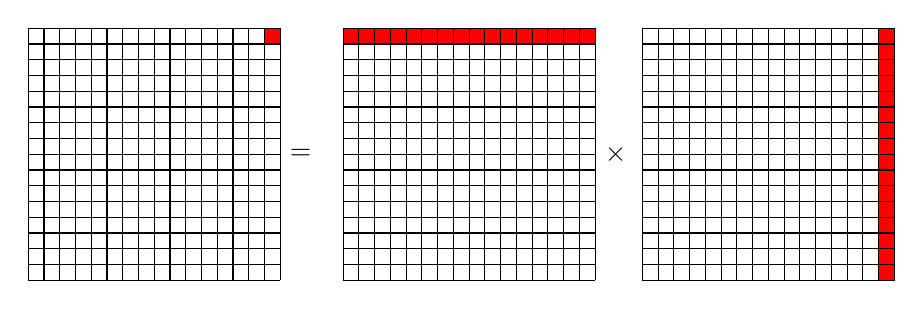
\begin{tikzpicture}[scale=0.2]
    \begin{scope}
      \draw[fill=red] (15,15)  rectangle (16,16);
      \draw[fill=red] (20,15) rectangle (36,16);
      \draw[fill=red] (54,0)  rectangle (55,16);
      \draw(0,0) grid(16,16);
      \draw(20,0) grid(36,16);
      \draw(39,0) grid(55,16);
      \node[right] at (16,8) {$=$};
      \node[right] at (36,8) {$\times$};
    \end{scope}
  \end{tikzpicture}
  \end{center}

\end{frame}

\begin{frame}
  \frametitle{Matmul: Outer product version}

  $C$ is a sum of outer products of columns of $A$ and rows of $B$.
  \begin{center}
  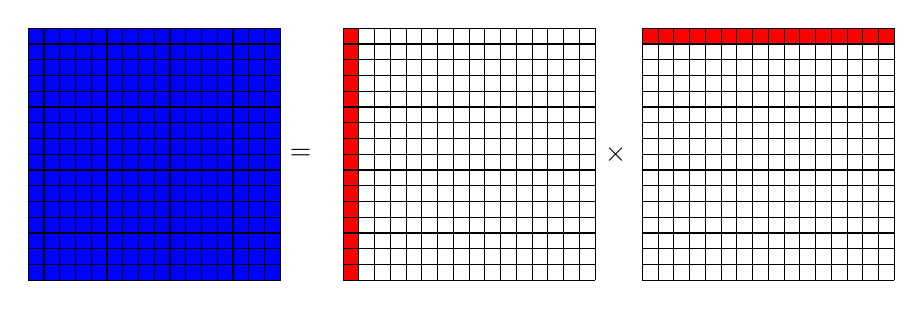
\begin{tikzpicture}[scale=0.2]
    \begin{scope}
      \draw[fill=blue] (0,0)  rectangle (16,16);
      \draw[fill=red] (20,0) rectangle (21,16);
      \draw[fill=red] (39,15)  rectangle (55,16);
      \draw(0,0) grid(16,16);
      \draw(20,0) grid(36,16);
      \draw(39,0) grid(55,16);
      \node[right] at (16,8) {$=$};
      \node[right] at (36,8) {$\times$};
    \end{scope}
  \end{tikzpicture}
  \end{center}

\end{frame}

\begin{frame}
  \frametitle{Matmul: Row-by-row}

  A row in $C$ is a row of $A$ multiplied by $B$.
  \begin{center}
  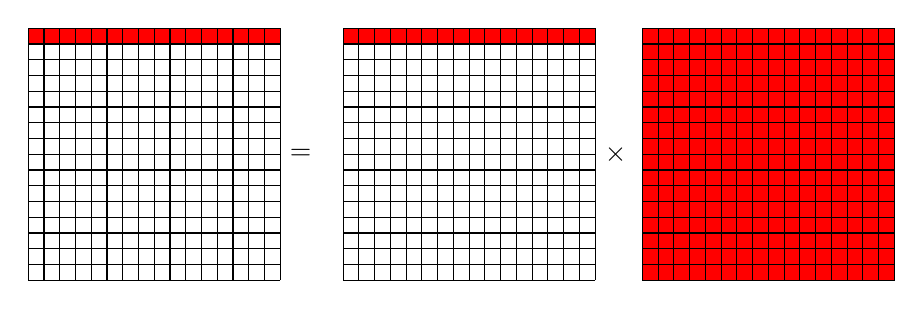
\begin{tikzpicture}[scale=0.2]
    \begin{scope}
      \draw[fill=red] (0,15)  rectangle (16,16);
      \draw[fill=red] (20,15) rectangle (36,16);
      \draw[fill=red] (39,0)  rectangle (55,16);
      \draw(0,0) grid(16,16);
      \draw(20,0) grid(36,16);
      \draw(39,0) grid(55,16);
      \node[right] at (16,8) {$=$};
      \node[right] at (36,8) {$\times$};
    \end{scope}
  \end{tikzpicture}
  \end{center}
  
\end{frame}


\begin{frame}
  \frametitle{Matmul: Col-by-col}

  A column in $C$ is $A$ multiplied by a column of $B$.
  \begin{center}
  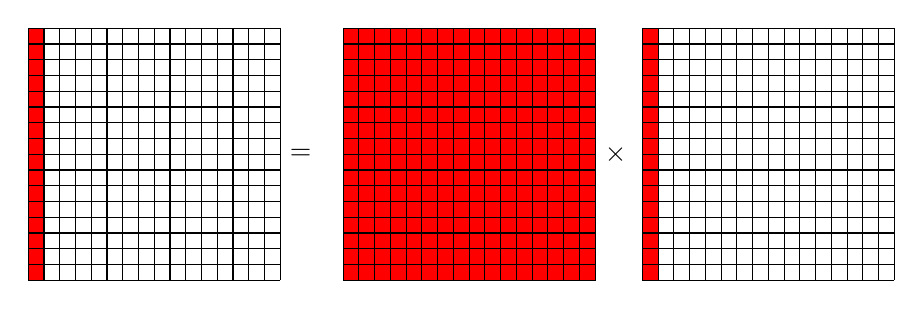
\begin{tikzpicture}[scale=0.2]
    \begin{scope}
      \draw[fill=red] (0,0)  rectangle (1,16);
      \draw[fill=red] (20,0) rectangle (36,16);
      \draw[fill=red] (39,0)  rectangle (40,16);
      \draw(0,0) grid(16,16);
      \draw(20,0) grid(36,16);
      \draw(39,0) grid(55,16);
      \node[right] at (16,8) {$=$};
      \node[right] at (36,8) {$\times$};
    \end{scope}
  \end{tikzpicture}
  \end{center}
  
\end{frame}

\begin{frame}
  \frametitle{Reality intervenes}

  These arrangements of matmul are theoretically equivalent. \\
  What about in practice? \\[5mm]
  Answer: Big differences due to {\em memory hierarchy}.
\end{frame}

\begin{frame}
  \frametitle{One row in naive matmul}

  \begin{center}
  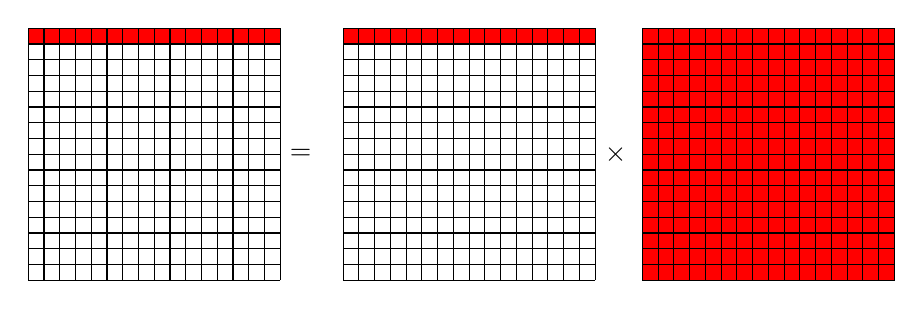
\begin{tikzpicture}[scale=0.2]
    \begin{scope}
      \draw[fill=red] (0,15)  rectangle (16,16);
      \draw[fill=red] (20,15) rectangle (36,16);
      \draw[fill=red] (39,0)  rectangle (55,16);
      \draw(0,0) grid(16,16);
      \draw(20,0) grid(36,16);
      \draw(39,0) grid(55,16);
      \node[right] at (16,8) {$=$};
      \node[right] at (36,8) {$\times$};
    \end{scope}
  \end{tikzpicture}
  \end{center}

  \begin{itemize}
  \item Access $A$ and $C$ with stride of $8M$ bytes
  \item Access {\em all} $8M^2$ bytes of $B$ before first re-use
  \item Poor {\em arithmetic intensity}
  \end{itemize}
\end{frame}

\begin{frame}
  \frametitle{Engineering strategy: blocking/tiling}

  \begin{center}
  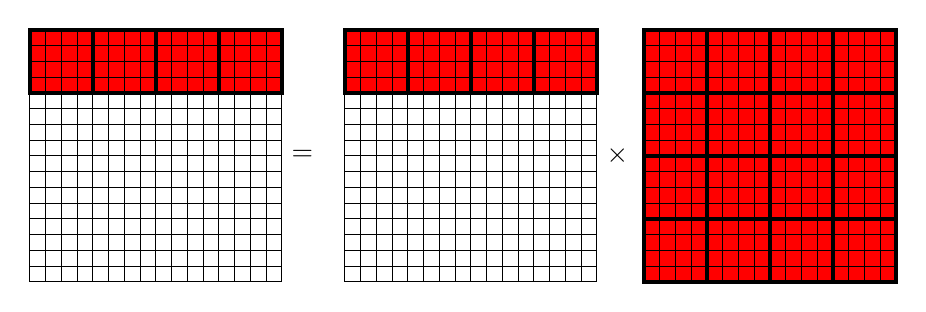
\begin{tikzpicture}[scale=0.2]
    \begin{scope}
      \foreach \i in {0,...,3}{
        \draw[fill=red,ultra thick] (4*\i,12) rectangle (4*\i+4,16);
       }
      \draw[fill=red] (20,15) rectangle (36,16);
      \foreach \i in {0,...,3}{
        \draw[fill=red,ultra thick] (20+4*\i,12) rectangle (20+4*\i+4,16);
       }
      \foreach \i in {0,...,3}{
        \foreach \j in {0,...,3}{
          \draw[fill=red,ultra thick] (39+4*\i,4*\j) rectangle (43+4*\i,4*\j+4);
        }
       }
      \draw(0,0) grid(16,16);
      \draw(20,0) grid(36,16);
      \draw(39,0) grid(55,16);
      \node[right] at (16,8) {$=$};
      \node[right] at (36,8) {$\times$};
    \end{scope}
  \end{tikzpicture}
  \end{center}

\end{frame}

\begin{frame}
  \frametitle{Simple model}

  Consider two types of memory (fast and slow) over which we have
  complete control.
  \begin{itemize}
  \item $m$ = words read from slow memory
  \item $t_m$ = slow memory op time
  \item $f$ = number of flops
  \item $t_f$ = time per flop
  \item $q = f/m$ = average flops / slow memory access
  \end{itemize}
  Time:
  \[
    f t_f + m t_m = f t_f \left( 1 + \frac{t_m/t_f}{q} \right)
  \]
  Larger $q$ means better time.
\end{frame}


\begin{frame}
  \frametitle{How big can $q$ be?}

  \begin{enumerate}
  \item Dot product: $n$ data, $2n$ flops
  \item Matrix-vector multiply: $n^2$ data, $2n^2$ flops
  \item Matrix-matrix multiply: $2n^2$ data, $2n^3$ flops
  \end{enumerate}
  These are examples of level 1, 2, and 3 routines in
  {\em Basic Linear Algebra Subroutines} (BLAS).
  We like building things on level 3 BLAS routines.

\end{frame}


\begin{frame}
  \frametitle{$q$ for naive matrix multiply}

  $q \approx 2$ (on board)
\end{frame}

\begin{frame}
  \frametitle{$q$ for blocked matrix multiply}

  $q \approx b$ (on board).  If $M_f$ words of fast memory,
  $b \approx \sqrt{M_f/3}$.

\vspace{1cm}
  Th: (Hong/Kung 1984, Irony/Tishkin/Toledo 2004):
  Any reorganization of this algorithm that uses only associativity
  and commutativity of addition is limited to $q = O(\sqrt{M_f})$

\vspace{1cm}
  Note: Strassen uses distributivity...
\end{frame}


\begin{frame}
  \frametitle{Concluding thoughts}

  \begin{itemize}
  \item Will not focus on performance {\em details} here (see CS 5220!)
  \item Knowing ``big picture'' issues makes a big difference
    \begin{itemize}
    \item Order-of-magnitude improvements through blocking ideas
    \item Even more possible through appropriate use of structure
    \end{itemize}
  \item Next time: More theoretical stuff!
  \end{itemize}
\end{frame}

\end{document}
